%%%%%%%%%%%%%%%%%%%%%%%%%%%%%%%%%%%%%%%%%%%%%%%%%%%%%%%%%%%%%%%%%%%%%%%%%%%%%%%%
\chapter{Проектирование аспектно-ориентированного расширения для языка Kotlin}
\label{cha:extension_design}
%%%%%%%%%%%%%%%%%%%%%%%%%%%%%%%%%%%%%%%%%%%%%%%%%%%%%%%%%%%%%%%%%%%%%%%%%%%%%%%%
Проектируемое расширение можно условно разделить на три части:
\begin{enumerate}
	\item Часть, отвечающая за анализ файлов с описанием аспектов и построения
		модели аспектов.
	\item Часть, отвечающая за построение PSI и его компиляцию в байт-код.
	\item Часть, отвечающая за внедрение аспектов в целевую программу.
\end{enumerate}
%%%%%%%%%%%%%%%%%%%%%%%%%%%%%%%%%%%%%%%%%%%%%%%%%%%%%%%%%%%%%%%%%%%%%%%%%%%%%%%%
\section{Структура программной системы}
\label{sec:prototype_structure}
%%%%%%%%%%%%%%%%%%%%%%%%%%%%%%%%%%%%%%%%%%%%%%%%%%%%%%%%%%%%%%%%%%%%%%%%%%%%%%%%
Перед проектированием структуры будущей системы, необходимо выбрать способ
внедрения аспектов.
Ввиду того, что внедрение аспектов при помощи прокси-объектов может значительно
ухудшить быстродействие системы, а при анализе байт-кода невозможно выделить
ряд специфичных для языка Kotlin языковых конструкций, было решено использовать
статический способ применения аспектов.
Внедрение аспектов сразу после компиляции является трудным в реализации, по
причинам, описанным выше.
При анализе, непосредственно, исходных кодов программы необходимо реализовывать
грамматику языка Kotlin, что также требует больших затрат.
Исходя из этих причин, было решено внедрять аспекты непосредственно в процессе
компиляции, путем модификации промежуточного представления программы.

После анализа поставленной задачи и существующих на данных момент
АОП-расширений, была предложена следующая архитектура программной системы,
представленная на рисунке~\ref{fig:program_architecture}.

\begin{figure}[htbp]
\centering
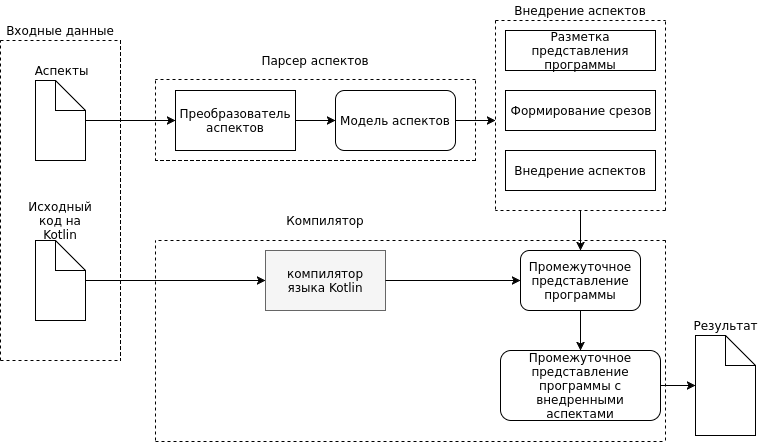
\includegraphics[width=\textwidth]{fig/program_architecture}
\caption{Архитектура программной системы}%
\label{fig:program_architecture}
\end{figure}

Как видно из рисунка~\ref{fig:program_architecture}, система состоит из
следующих частей:
\begin{enumerate}
	\item Первой частью системы являются преобразователи, отвечающие за
		 импортирование исходного кода и описания аспектов и приведения их к
		 виду промежуточного представления.
		 Для создания преобразователя аспектов, необходимо сформировать
		 грамматику описания аспектов.
		 Создание промежуточного представления программы может быть переложено
		 на компилятор языка Kotlin.
	\item Второй частью системы является часть, отвечающая за внедрение аспектов
		в промежуточное представление программы.
		Данная часть состоит из нескольких компонентов: части, отвечающей за
		разметку промежуточного представления, части, отвечающей за формирование
		срезов и части, реализующей внедрение аспектов.
	\item Последней частью системы является часть, отвечающая за компиляцию
		модифицированного промежуточного представления программы в байт-код.
		Данную часть также нет необходимости реализовывать полностью самому, так
		как можно воспользоваться готовыми системами сборки, передав в них
		не исходные коды программы, а модифицированное промежуточное
		представление.
\end{enumerate}

Таким образом, основное внимание стоит уделить модулям, отвечающим за построение
модели аспектов и внедрению аспектов в промежуточное представление программы.
%%%%%%%%%%%%%%%%%%%%%%%%%%%%%%%%%%%%%%%%%%%%%%%%%%%%%%%%%%%%%%%%%%%%%%%%%%%%%%%%
\section{Разработка синтаксиса аспектов}
\label{sec:aspect_syntax_design}
%%%%%%%%%%%%%%%%%%%%%%%%%%%%%%%%%%%%%%%%%%%%%%%%%%%%%%%%%%%%%%%%%%%%%%%%%%%%%%%%
По результатам анализа существующих АОП-расширений можно выделить два основных
способа описания аспектов: создание классов, каждый из которых позволяет
производить вставку кода советов или же использование дополнительного синтаксиса
описания аспектов.
Для разрабатываемого прототипа был выбран второй способ, а именно, создание
отдельного синтаксиса описания аспектов, схожего с описанием классов в языке
Kotlin.

За основу разрабатываемого синтаксиса было решено взять язык описания аспектов,
используемый в фреймворке AspectJ.
Данный выбор был сделан, во-первых, из-за большой популярности данного
АОП-расширения и, во-вторых, из-за удобства и гибкости данного способа описания
аспектов.
%%%%%%%%%%%%%%%%%%%%%%%%%%%%%%%%%%%%%%%%%%%%%%%%%%%%%%%%%%%%%%%%%%%%%%%%%%%%%%%%
\subsection{Синтаксис описания аспекта}
\label{sub:custom_aspect_syntax}
%%%%%%%%%%%%%%%%%%%%%%%%%%%%%%%%%%%%%%%%%%%%%%%%%%%%%%%%%%%%%%%%%%%%%%%%%%%%%%%%
Как и в AspectJ, сквозная функциональность инкапсулируется в сущности,
называемой \textit{аспект}.
Каждый аспект имеет свой уникальный идентификатор и может содержать как описание
советов и срезов, так и переменные и функции, предназначенные для внутреннего
использование.
Описание аспекта, в целом, похоже на описание класса в языке Kotlin: оно
начинается с ключевого слова \textit{aspect}, после чего следует идентификатор
аспекта и, затем, тело аспекта, заключенное в фигурные скобки.
Пример описания аспекта с идентификатором \textit{FooAspect} приведен в листинге
~\ref{lst:custom_aspect_example}.
  \begin{lstlisting}[language=Java, label={lst:custom_aspect_example}, 
  caption={Пример описания аспекта в разрабатываемом прототипе}]
aspect FooAspect  {
  ... Тело аспекта
}
  \end{lstlisting}
%%%%%%%%%%%%%%%%%%%%%%%%%%%%%%%%%%%%%%%%%%%%%%%%%%%%%%%%%%%%%%%%%%%%%%%%%%%%%%%%
\subsection{Синтаксис описания срезов}
\label{sub:custom_pointcut_syntax}
%%%%%%%%%%%%%%%%%%%%%%%%%%%%%%%%%%%%%%%%%%%%%%%%%%%%%%%%%%%%%%%%%%%%%%%%%%%%%%%%
За основу синтаксиса описания срезов был также взят фреймворк AspectJ.
Описание среза начинается с ключевого слова \textit{pointcut}, после чего
следует идентификатор среза, уникальный в рамках данного аспекта, перечень
аргументов и, непосредственно, описание среза.
При описании среза могут использоваться следующие конструкции:
\begin{itemize}
	\item \textit{call(паттерн\_метода)} --- вызов метода, указанного в
		  описании.
	\item \textit{execution(паттерн\_метода)} --- выполнение метода,
		  указанного в описании.
\end{itemize}

Описание метода также состоит из нескольких частей, описанных ниже в порядке их
следования:
\begin{enumerate}
	\item \textit{аннотации метода} --- необязательный параметр, содержащий
		  список аннотаций.
		  Можно задавать как обязательное наличие, так и отсутствие определенной
		  аннотации при помощи символа \quotes{!}.
	\item \textit{модификаторы метода} --- необязательный параметр, содержащий
		  описание модификаторов метода.
		  Может принимать следующие значения: public, private, protected,
		  internal, synchronized, final.
		  Можно задавать как обязательное наличие, так и отсутствие какого-либо
		  модификатора при помощи символа \quotes{!}.
	\item \textit{extension модификатор} --- необязательный параметр, задающий,
		  является ли функция \quotes{расширением} или нет.
	\item ключевое слово \quotes{fun}.
	\item \textit{название пакета} --- необязательный параметр, задающий имя
		  пакета и класса, в котором объявлена функция.
		  Возможен пропуск одного или нескольких символов, при помощи символа
		  \quotes{*}.
	\item \textit{имя функции} --- обязательный параметр, задающий имя функции.
		  Возможен пропуск одного или нескольких символов, при помощи символа
		  \quotes{*}.
	\item \textit{список типов параметров функции} --- необязательны параметр,
		  задающий список типов аргументов, которые имеет функция, в
		  соответствующем порядке.
		  В качестве типов, могут использоваться как стандартные типы языка
		  Kotlin, как, например, Double, Int, Short и т.д., так и
		  пользовательские типы данных.
		  Опционально можно указывать соответствие параметров функции на
		  \quotes{NotNull} и \quotes{Nullable} при помощи модификаторов
		  \quotes{!!} и \quotes{?} соответственно.
		  Если количество и типы аргументов функции не имеет значения, то это
		  можно указать, используя символ \quotes{..}.
		  Список параметров оборачивается в круглые скобки.
	\item \textit{тип возвращаемого значения} --- необязательный параметр,
		  показывающий тип значения, возвращаемого функцией.
		  В качестве типа, могут использоваться как стандартные типы языка
		  Kotlin, как, например, Double, Int, Short и т.д., так и
		  пользовательские типы данных.
		  Также как и при указании параметров функции, типу возвращаемого
		  значения можно задавать соответствие на \quotes{NotNull} и
		  \quotes{Nullable} при помощи модификаторов \quotes{!!} и \quotes{?}.
		  При указании типа возвращаемого значения, оно отделяется от списка
		  аргументов символом \quotes{:}, по аналогии с описанием функций на
		  языке Kotlin.
\end{enumerate}

Данные конструкции могут группироваться между собой при помощи следующих
логических операций \textit{конъюнкции} (\&\&),  \textit{дизъюнкции} (||)  и
\textit{инверсии} (!).
При описании срезов могут использоваться не только 
%%%%%%%%%%%%%%%%%%%%%%%%%%%%%%%%%%%%%%%%%%%%%%%%%%%%%%%%%%%%%%%%%%%%%%%%%%%%%%%%
\subsection{Синтаксис описания советов}
\label{sub:custom_advice_syntax}
%%%%%%%%%%%%%%%%%%%%%%%%%%%%%%%%%%%%%%%%%%%%%%%%%%%%%%%%%%%%%%%%%%%%%%%%%%%%%%%%
Описание советов также во многом схоже с описанием, используемым в AspectJ.
Оно начинается с ключевого слова, описывающего способ внедрения
кода совета относительно точки объединения, а именно:
\begin{itemize}
	\item \textit{before} --- вставка кода совета до точки объединения;
	\item \textit{after} --- вставка кода совета после точки объединения;
	\item \textit{around} --- вставка кода совета до и после точки объединения;
\end{itemize}
После этого могут следовать аргументы функций, к которым будет производиться
обращение внутри кода совета.

Следующей частью совета является описание среза, аналогичное представленному в
разделе~\ref{sub:custom_pointcut_syntax}, после которого следует код совета,
представляющий из себя программный код на языке Kotlin.
%%%%%%%%%%%%%%%%%%%%%%%%%%%%%%%%%%%%%%%%%%%%%%%%%%%%%%%%%%%%%%%%%%%%%%%%%%%%%%%%
\section{Выводы}
\label{sec:design_conclusion}
%%%%%%%%%%%%%%%%%%%%%%%%%%%%%%%%%%%%%%%%%%%%%%%%%%%%%%%%%%%%%%%%%%%%%%%%%%%%%%%%
%%%%%%%%%%%%%%%%%%%%%%%%%%%%%%%%%%%%%%%%%%%%%%%%%%%%%%%%%%%%%%%%%%%%%%%%%%%%%%%%
